% Options for packages loaded elsewhere
\PassOptionsToPackage{unicode}{hyperref}
\PassOptionsToPackage{hyphens}{url}
%
\documentclass[
  english,
  ,doc,floatsintext]{apa6}
\usepackage{lmodern}
\usepackage{amssymb,amsmath}
\usepackage{ifxetex,ifluatex}
\ifnum 0\ifxetex 1\fi\ifluatex 1\fi=0 % if pdftex
  \usepackage[T1]{fontenc}
  \usepackage[utf8]{inputenc}
  \usepackage{textcomp} % provide euro and other symbols
\else % if luatex or xetex
  \usepackage{unicode-math}
  \defaultfontfeatures{Scale=MatchLowercase}
  \defaultfontfeatures[\rmfamily]{Ligatures=TeX,Scale=1}
\fi
% Use upquote if available, for straight quotes in verbatim environments
\IfFileExists{upquote.sty}{\usepackage{upquote}}{}
\IfFileExists{microtype.sty}{% use microtype if available
  \usepackage[]{microtype}
  \UseMicrotypeSet[protrusion]{basicmath} % disable protrusion for tt fonts
}{}
\makeatletter
\@ifundefined{KOMAClassName}{% if non-KOMA class
  \IfFileExists{parskip.sty}{%
    \usepackage{parskip}
  }{% else
    \setlength{\parindent}{0pt}
    \setlength{\parskip}{6pt plus 2pt minus 1pt}}
}{% if KOMA class
  \KOMAoptions{parskip=half}}
\makeatother
\usepackage{xcolor}
\IfFileExists{xurl.sty}{\usepackage{xurl}}{} % add URL line breaks if available
\IfFileExists{bookmark.sty}{\usepackage{bookmark}}{\usepackage{hyperref}}
\hypersetup{
  pdftitle={Covid-19: Stalking},
  hidelinks,
  pdfcreator={LaTeX via pandoc}}
\urlstyle{same} % disable monospaced font for URLs
\usepackage{graphicx,grffile}
\makeatletter
\def\maxwidth{\ifdim\Gin@nat@width>\linewidth\linewidth\else\Gin@nat@width\fi}
\def\maxheight{\ifdim\Gin@nat@height>\textheight\textheight\else\Gin@nat@height\fi}
\makeatother
% Scale images if necessary, so that they will not overflow the page
% margins by default, and it is still possible to overwrite the defaults
% using explicit options in \includegraphics[width, height, ...]{}
\setkeys{Gin}{width=\maxwidth,height=\maxheight,keepaspectratio}
% Set default figure placement to htbp
\makeatletter
\def\fps@figure{htbp}
\makeatother
\setlength{\emergencystretch}{3em} % prevent overfull lines
\providecommand{\tightlist}{%
  \setlength{\itemsep}{0pt}\setlength{\parskip}{0pt}}
\setcounter{secnumdepth}{5}
% Make \paragraph and \subparagraph free-standing
\ifx\paragraph\undefined\else
  \let\oldparagraph\paragraph
  \renewcommand{\paragraph}[1]{\oldparagraph{#1}\mbox{}}
\fi
\ifx\subparagraph\undefined\else
  \let\oldsubparagraph\subparagraph
  \renewcommand{\subparagraph}[1]{\oldsubparagraph{#1}\mbox{}}
\fi
% Manuscript styling
\usepackage{upgreek}
\captionsetup{font=singlespacing,justification=justified}

% Table formatting
\usepackage{longtable}
\usepackage{lscape}
% \usepackage[counterclockwise]{rotating}   % Landscape page setup for large tables
\usepackage{multirow}		% Table styling
\usepackage{tabularx}		% Control Column width
\usepackage[flushleft]{threeparttable}	% Allows for three part tables with a specified notes section
\usepackage{threeparttablex}            % Lets threeparttable work with longtable

% Create new environments so endfloat can handle them
% \newenvironment{ltable}
%   {\begin{landscape}\begin{center}\begin{threeparttable}}
%   {\end{threeparttable}\end{center}\end{landscape}}
\newenvironment{lltable}{\begin{landscape}\begin{center}\begin{ThreePartTable}}{\end{ThreePartTable}\end{center}\end{landscape}}

% Enables adjusting longtable caption width to table width
% Solution found at http://golatex.de/longtable-mit-caption-so-breit-wie-die-tabelle-t15767.html
\makeatletter
\newcommand\LastLTentrywidth{1em}
\newlength\longtablewidth
\setlength{\longtablewidth}{1in}
\newcommand{\getlongtablewidth}{\begingroup \ifcsname LT@\roman{LT@tables}\endcsname \global\longtablewidth=0pt \renewcommand{\LT@entry}[2]{\global\advance\longtablewidth by ##2\relax\gdef\LastLTentrywidth{##2}}\@nameuse{LT@\roman{LT@tables}} \fi \endgroup}

% \setlength{\parindent}{0.5in}
% \setlength{\parskip}{0pt plus 0pt minus 0pt}

% \usepackage{etoolbox}
\makeatletter
\patchcmd{\HyOrg@maketitle}
  {\section{\normalfont\normalsize\abstractname}}
  {\section*{\normalfont\normalsize\abstractname}}
  {}{\typeout{Failed to patch abstract.}}
\makeatother
\shorttitle{Covid-19: Stalking}
\author{Orestis Kopsacheilis\textsuperscript{1}\ \& Lionel Roger\textsuperscript{2}}
\affiliation{
\vspace{0.5cm}
\textsuperscript{1} School of Economics, University of Nottingham\\\textsuperscript{2} ODI}
\usepackage{csquotes}
\usepackage{setspace, appendix, placeins}
\usepackage[justification=centering]{caption}
\usepackage{float}
\floatplacement{figure}{H}
\usepackage{xcolor}
\newcommand{\onote}[1]{{\color{blue} {(\sf Orestis:} {\sl{#1}}     {\sf )}}}
\newcommand{\lnote}[1]{{\color{green} {(\sf Lio:} {\sl{#1}}     {\sf )}}}
\newtheorem{finding}{Finding}
\ifxetex
  % Load polyglossia as late as possible: uses bidi with RTL langages (e.g. Hebrew, Arabic)
  \usepackage{polyglossia}
  \setmainlanguage[]{english}
\else
  \usepackage[shorthands=off,main=english]{babel}
\fi

\title{Covid-19: Stalking}

\date{16 May, 2020}

\abstract{
TBD
}

\begin{document}
\maketitle

{
\setcounter{tocdepth}{2}
\tableofcontents
}
\hypertarget{data-description}{%
\section{Data description}\label{data-description}}

Following a long process of collecting and compiling data, we are now in a position to claim that we basically have (or can easily obtain) every available information related to Covid-19 at a country level (and often in a more disaggregate level too).

We can summarise the data we are currently focusing on in four layers (always referring at the country level unless specified otherwise).

\begin{enumerate}
\def\labelenumi{\arabic{enumi}.}
\tightlist
\item
  Movement according to the Google reports.
\item
  Policy updates on a daily basis.
\item
  Summary statistics on Covid-19 deaths, total cases, tests, etc.
\item
  Economic indexes, demographics and behavioural measures
\end{enumerate}

\hypertarget{motivation}{%
\section{Motivation}\label{motivation}}

After a period of approximately 10 weeks of strict social distancing measures, several countries have started lifting such restrictions gradually.

\begin{itemize}
\tightlist
\item
  France: 11/05/2020
\item
  Germany: Munich reopens Biergartens from 18/05/2020
\item
  US: plan to reopen businesses over coming weeks
\item
  Greece: traffic bans were revoked
\item
  UK: \ldots{}
\end{itemize}

Given the medical consensus, this will most likely result to another spike in total cases in the near future, raising the death-count from Covid-19.
It is not clear what the long-term strategy for dealing with Corona is.
In fact, certain strategies, would only really work, if they were not explicitly communicated.
Therefore, part of the motivation for this report is to hypothesize what some possible strategies might be and track data in order to track which of these hypotheses is more likely implemented.

\hypertarget{hypothesized-policies-conceptual-specification.}{%
\section{Hypothesized policies: conceptual specification.}\label{hypothesized-policies-conceptual-specification.}}

\hypertarget{the-accordeon-policy}{%
\subsection{\texorpdfstring{The \enquote{accordeon-policy}}{The `accordeon-policy'}}\label{the-accordeon-policy}}

In a nutshell, this policy entails a pattern of \enquote{imposing - lifting - re-imposing - \ldots{}} restrictions.
This implies a constant flow of cases in the hospitals - up to the capacity of each country's health-care system (flattening the curve).
The goal of this policy is to:

\hypertarget{goals}{%
\subsubsection{Goals}\label{goals}}

\begin{enumerate}
\def\labelenumi{\arabic{enumi}.}
\tightlist
\item
  maintain a somewhat functional economy
\item
  reduce social/ behavioural fatigue
\item
  gradually achieve herd immunity.
\end{enumerate}

A nice summary of how this plan would look like in practice and under which circumstances it would work \href{https://twitter.com/iandonald_psych/status/1238518371651649538?s=19}{here}.

All three goals can be discussed and debated.

\hypertarget{assumptions}{%
\subsubsection{Assumptions}\label{assumptions}}

\begin{enumerate}
\def\labelenumi{\arabic{enumi}.}
\item
  Goal 1. relies on the assumption that the benefits of this partial re-opening the economy outweight outweigh the costs.
  {\color{blue} {(\sf Orestis:} {\sl{We briefly discussed about this point. I tend to agree that assumption a., is probably not too wild but do maintain some hesitations. You seemed more confident it holds.}}     {\sf )}}
  There must be several macro-economics-y papers providing models and assessments on the long-run implications of keeping the economy close vs.~semi-open etc.
  {\color{blue} {(\sf Orestis:} {\sl{I don't think we should be focussing on analysing this aspect.}}     {\sf )}}
\item
  Behavioural fatigue is eased by not having to withstand one prolongued period of isolation.
\end{enumerate}

Even if we assume that relaxing measures and re-introducing them does not increase the total amount people would need to spend under social isolation (SI), this assumption is dubbious. Not aware of any research (but perhaps worth doing a quick background check) but to the extend that the cost of SI is concave, i.e.~early days of isolation feel worse than later days, then pushing people repeatedly on that early part of the curve has an adverse effect.
It can be made worse. Just as you get used to the new lifestyle, you now go back to the previous one and then back again. Transition is more tiring.

\begin{enumerate}
\def\labelenumi{\arabic{enumi}.}
\setcounter{enumi}{2}
\item
  people's adherence to SI measures remains constant across iterations.
  Again, this is not necessarily the case. It could very well be that people adhere less and less (behavioural fatigue might be one of the reasons, especially if it is true that the transition from social life to SI is the hardest part).
\item
  Herd-immunity is realistic.
  This is a point that is better reserved for medical doctors.
\end{enumerate}

\hypertarget{empirical-identification}{%
\subsubsection{Empirical identification}\label{empirical-identification}}

Overall, the corona-net data-base is key here.
If the `accordeon policy' holds true, we should observe an oscilating pattern when plotting the policy restriction index over time.
Currently, according to Figure \ref{fig:ActIndex}, this oscilation happens very lightly on an increasing severity trend.
According to this hypothesis, we should expect this trend to flatten and the oscilation to intensify.

\begin{figure}
\centering
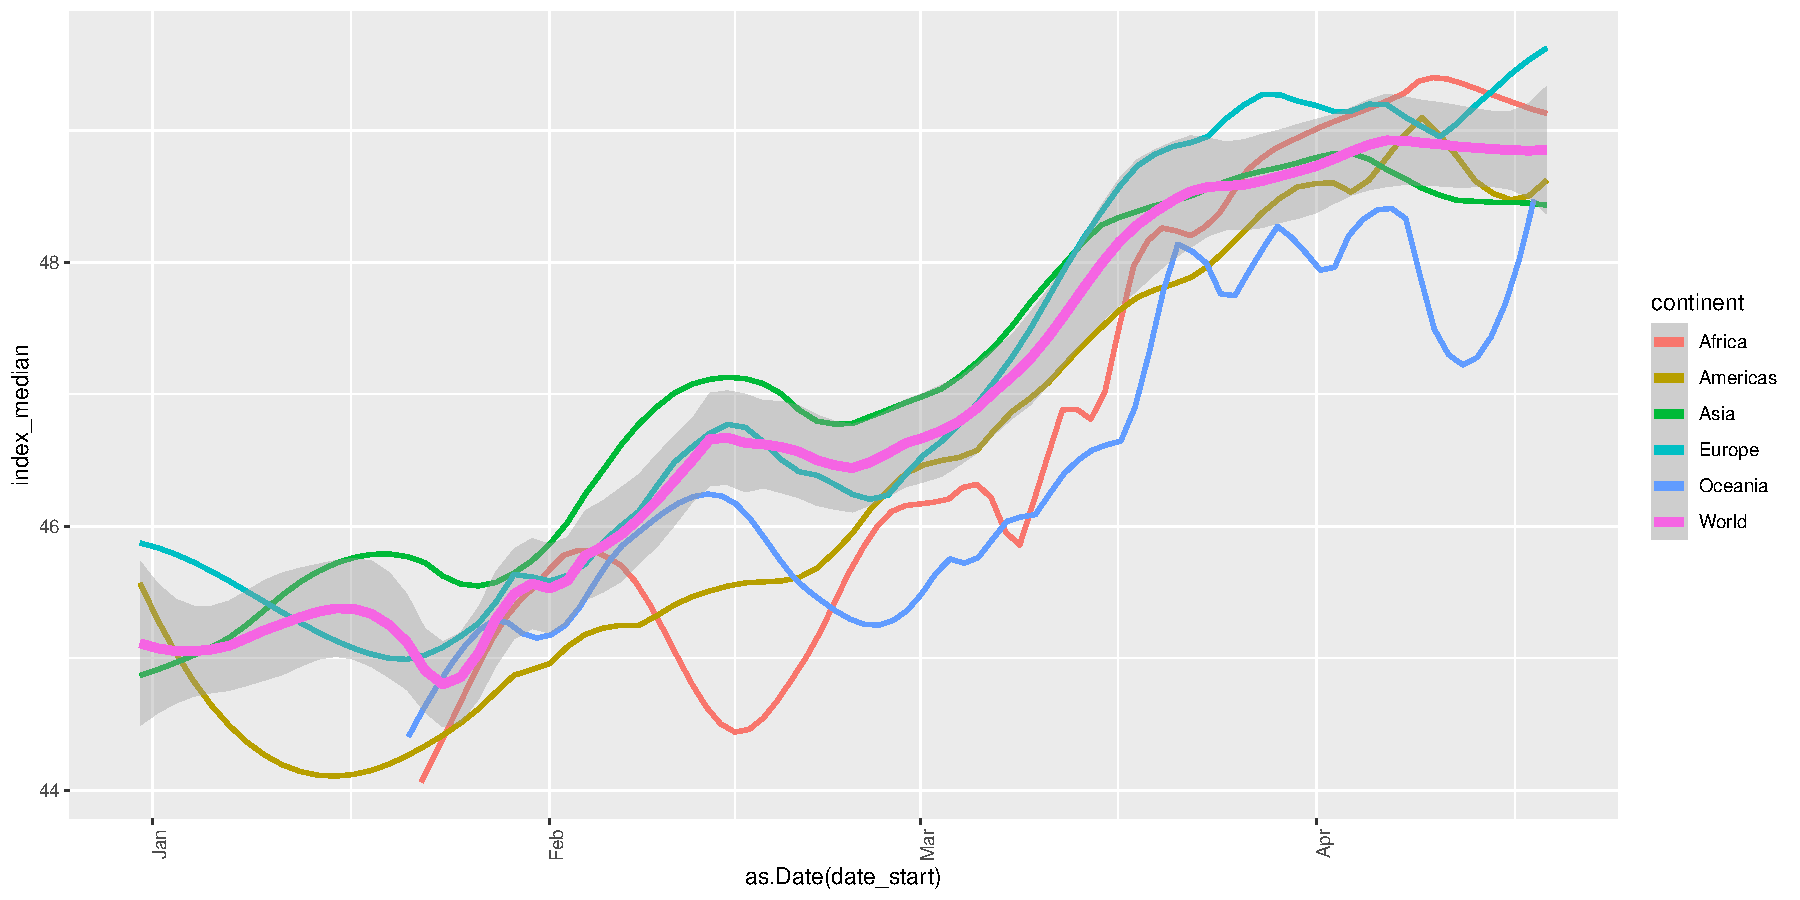
\includegraphics{covid-19_2_files/figure-latex/ActIndex-1.pdf}
\caption{\label{fig:ActIndex}Activity Index by Country}
\end{figure}

What about using data to assess the assumptions on which the success of the accordeon relies on?
I think that among the 3 assumptions, our focus is best emphasized on the second and third ones.
A challenging aspect of this is that the two assumptions are partially overlapping.
Behavioural fatigue (assumption 2) can be the key contributor for reduced adherence over later waves of restrictions.

For the behavioural fatigue assumption we can measure public's attitudes at different times: early on after the first SI measures, later on, right after the second wave of SI (has not yet come). \href{https://www.nber.org/papers/w27082}{This ongoing survey} might be a good source for tracking this.

\begin{figure}
\centering
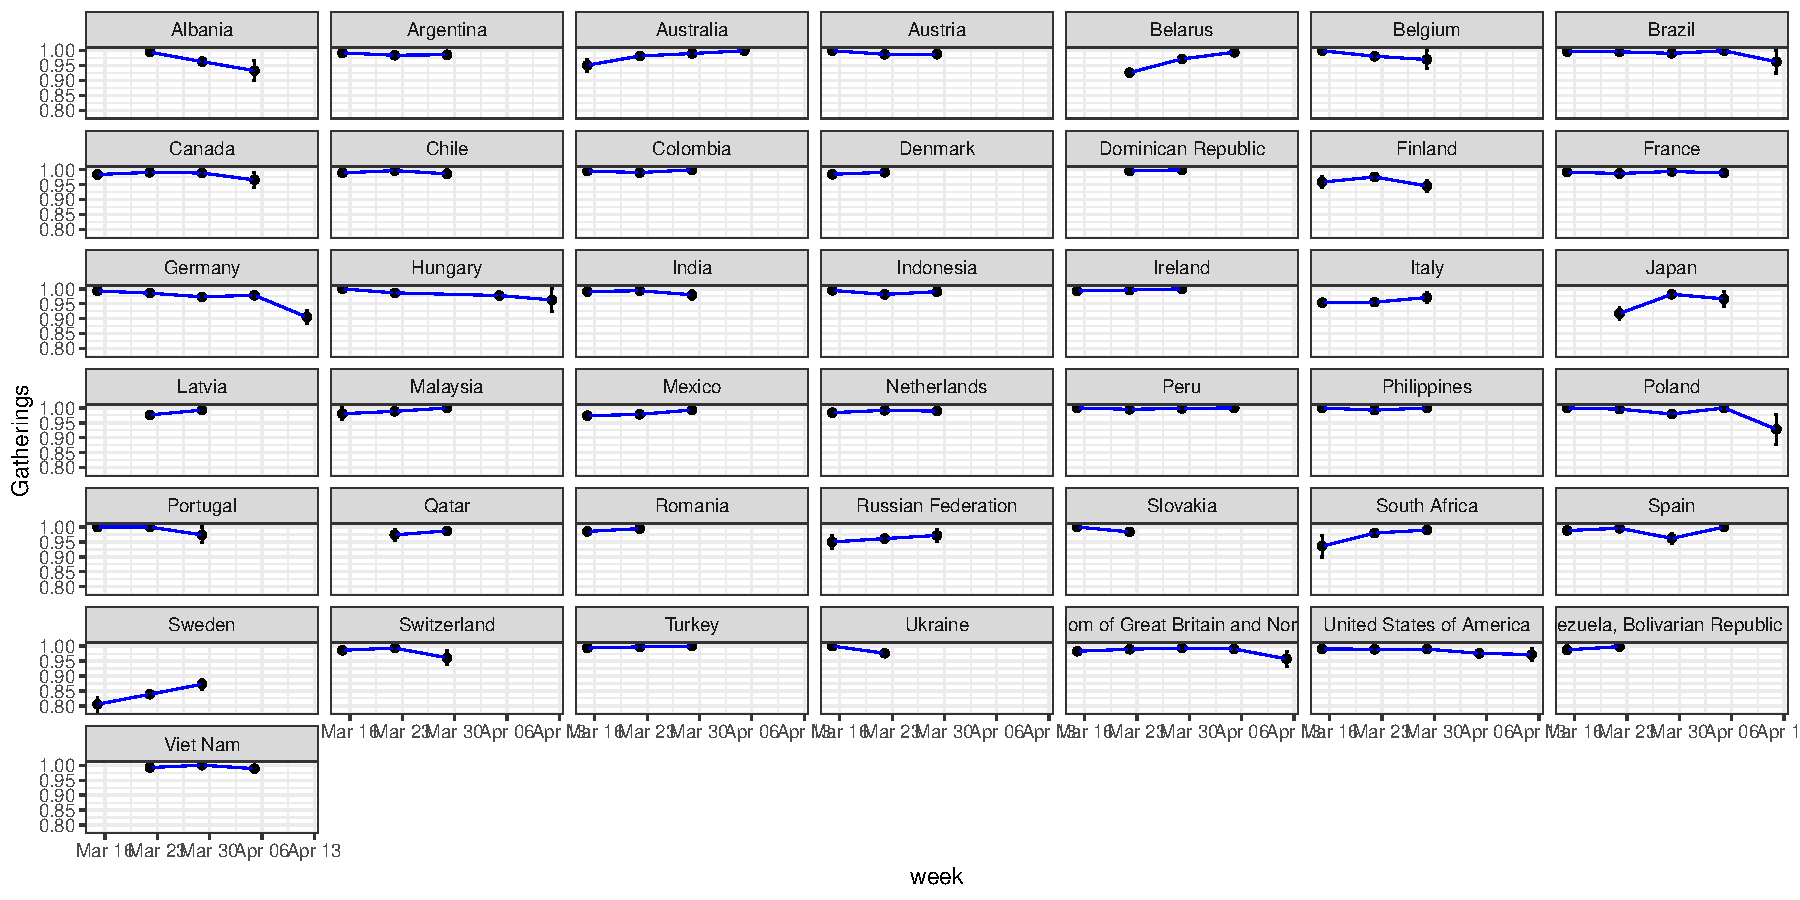
\includegraphics{covid-19_2_files/figure-latex/fobG-1.pdf}
\caption{\label{fig:fobG}Cancel social gatherings?}
\end{figure}

\begin{figure}
\centering
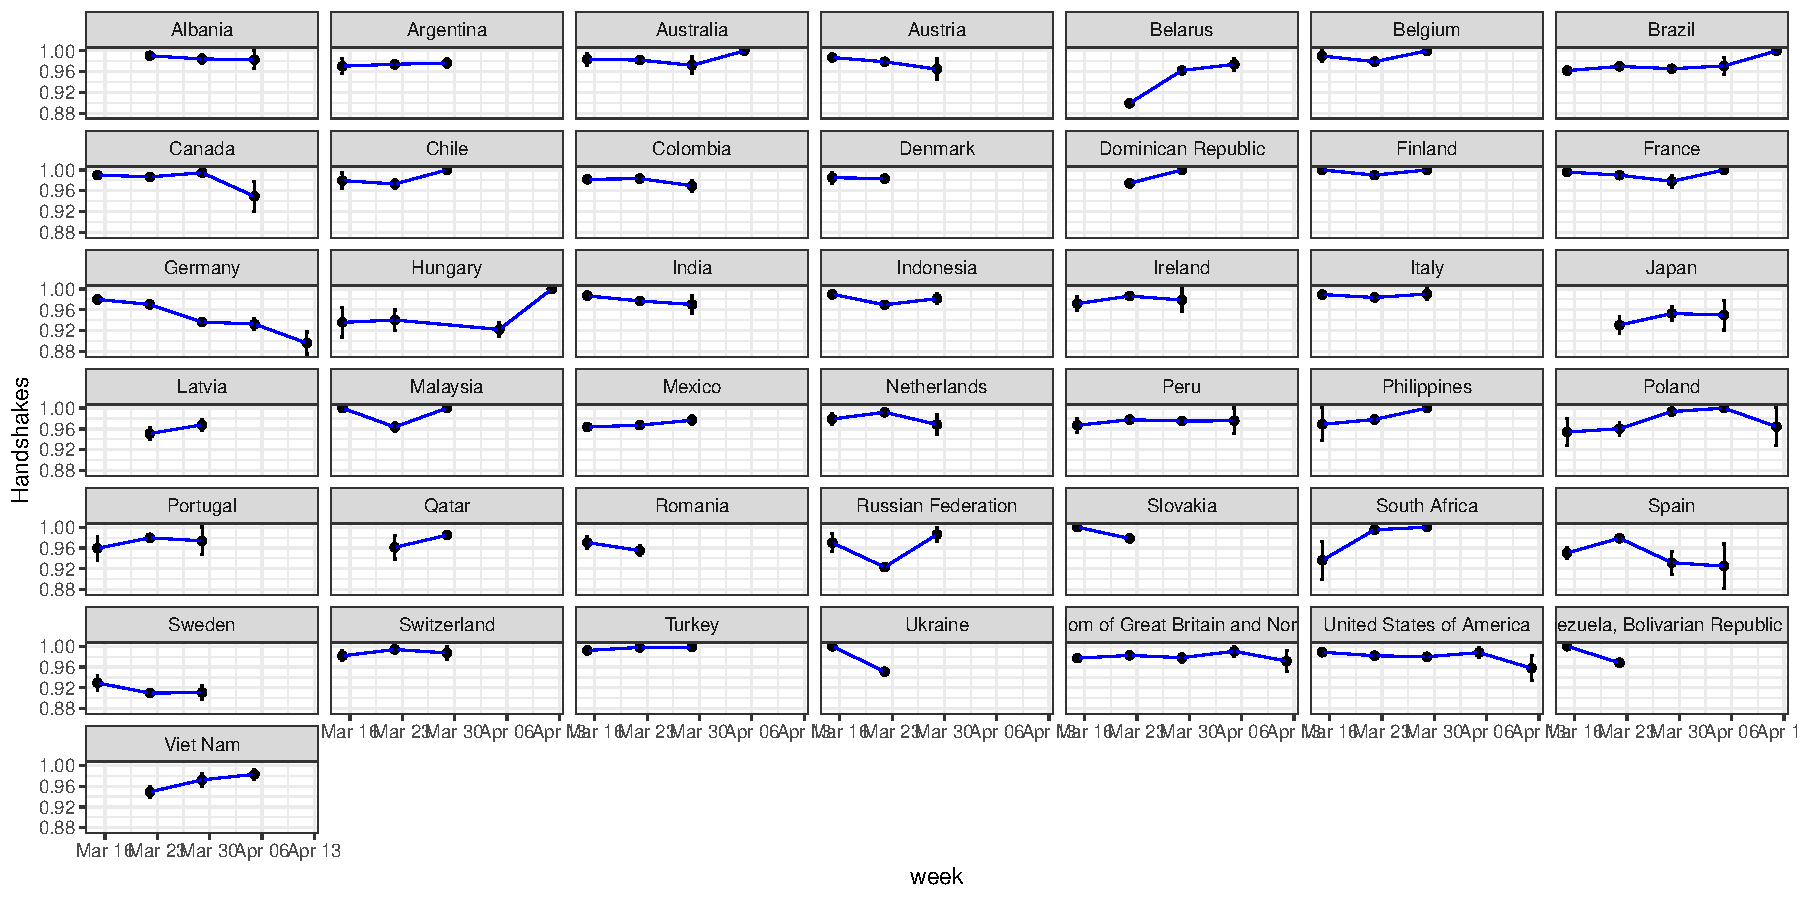
\includegraphics{covid-19_2_files/figure-latex/fobH-1.pdf}
\caption{\label{fig:fobH}Shake hands?}
\end{figure}

\begin{figure}
\centering
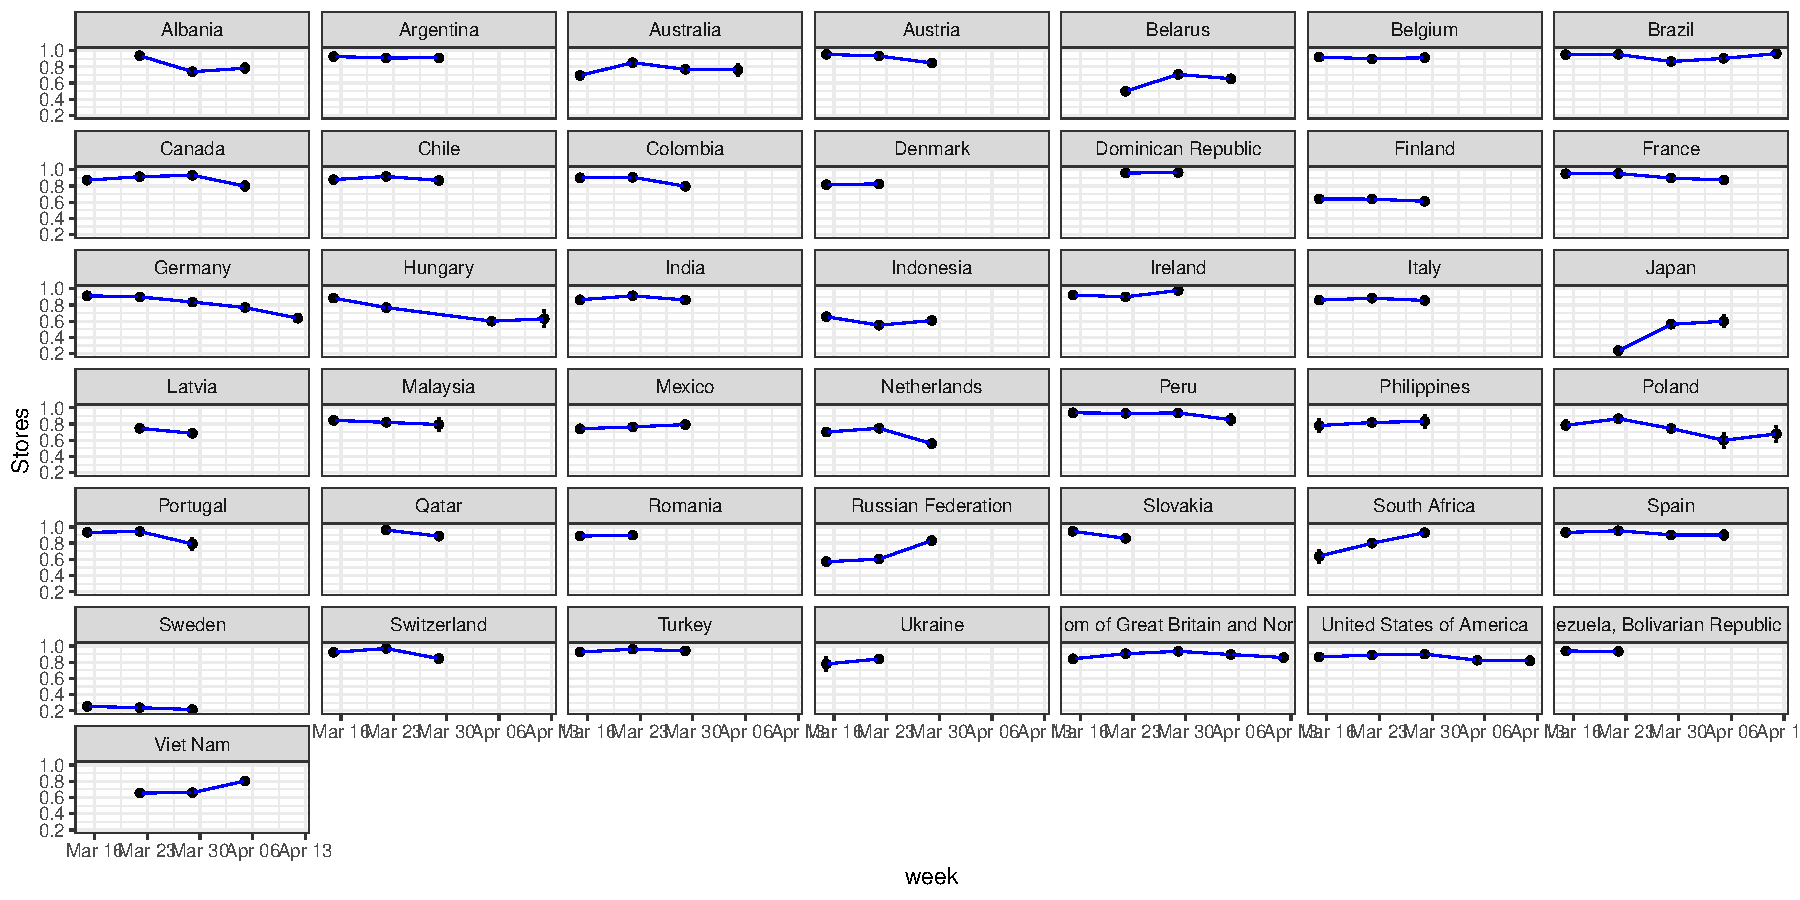
\includegraphics{covid-19_2_files/figure-latex/fobST-1.pdf}
\caption{\label{fig:fobST}Close stores?}
\end{figure}

\begin{figure}
\centering
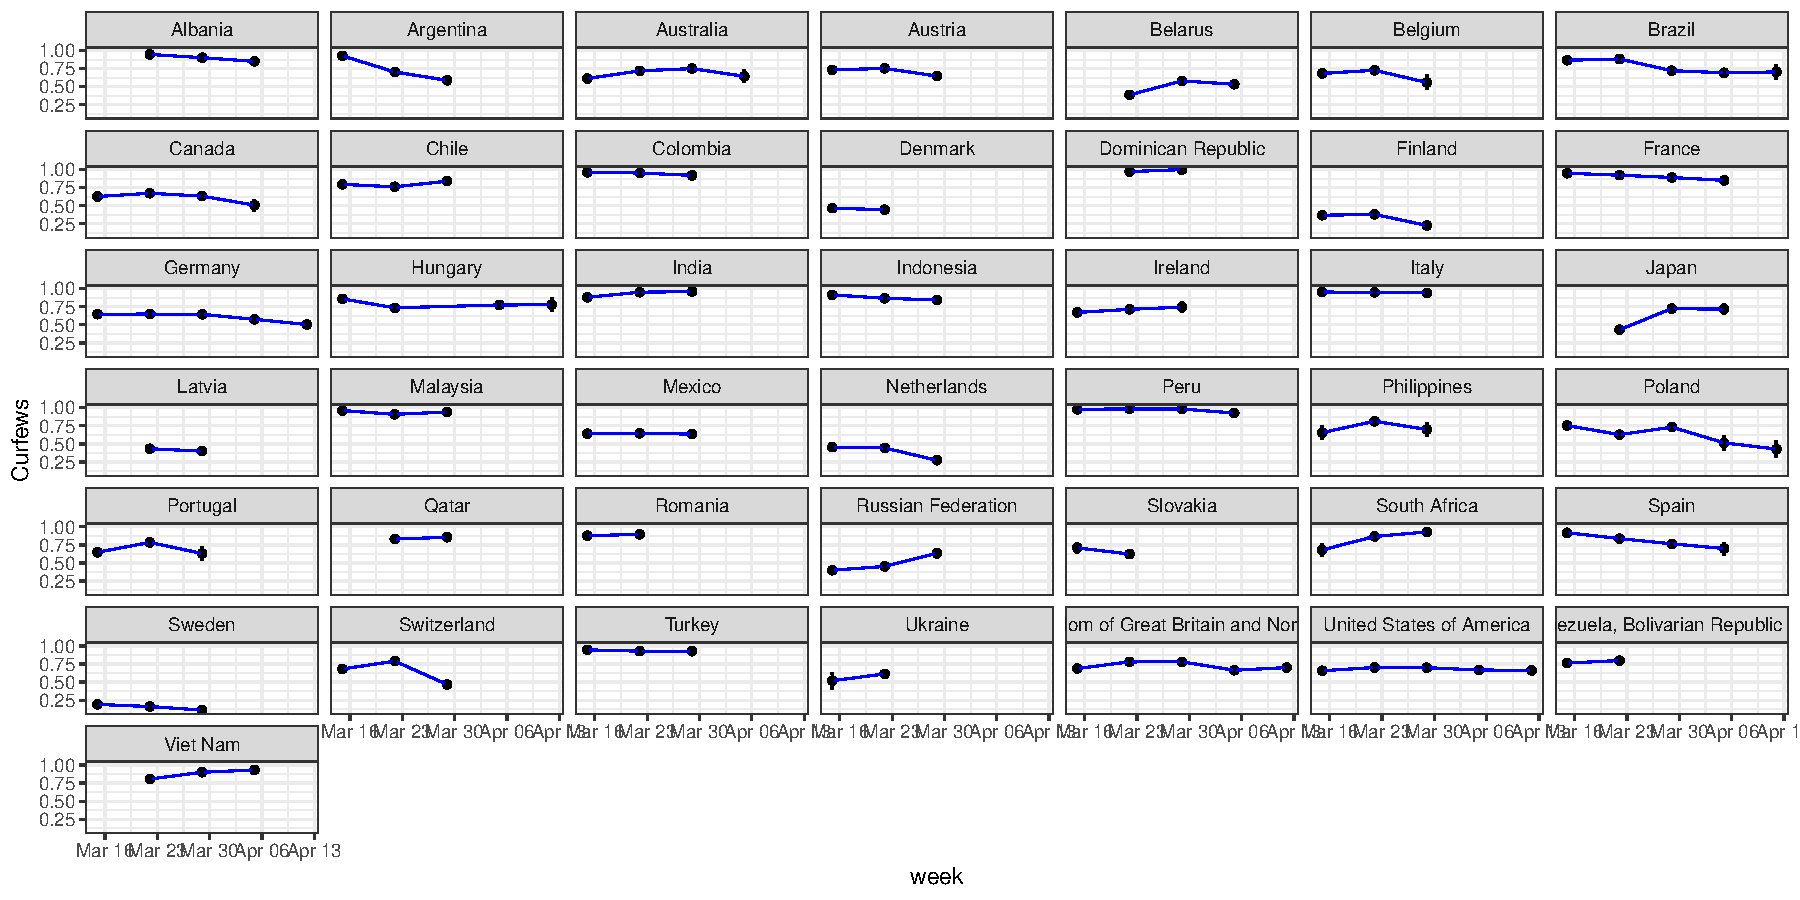
\includegraphics{covid-19_2_files/figure-latex/fobCRF-1.pdf}
\caption{\label{fig:fobCRF}Curfew}
\end{figure}

For the level of adherence the obvious choice would be to measure change in Google's movement right after the 2nd wave SI.
One interesting idea to investigate relates to measuring the \textbf{speed of increase in movement following relaxation of social distancing measures}.

\begin{itemize}
\tightlist
\item
  Is it symmetric to the speed of adhering to social distancing directives (but with different sign)?
\item
  What can we infer by the disparity between the adherence to social isolation measures and re-opening the economy directives?
\end{itemize}

\hypertarget{u-turn}{%
\subsection{U-turn}\label{u-turn}}

The course-correction. We realised that initial reactions were excessive. The virus is not as deadly. Or, perhaps, we realise that the current policy mixture might be worse in the long run. Measures are lifted without the intention to be re-implemented. Whoever dies, dies.

\hypertarget{crushing-the-curve}{%
\subsection{Crushing the curve}\label{crushing-the-curve}}

No-one dare leave his/her house until\ldots the end. Not sure what the end is in this case. It cannot be herd-immunity so it probably means, until a vaccine is developped, or a very efficient medication.

\hypertarget{strategic-planning-whos-doing-it}{%
\section{Strategic planning: who's doing it?}\label{strategic-planning-whos-doing-it}}

Didn't have time to develop this. Very briefly:

\begin{itemize}
\tightlist
\item
  Not all countries follow a deliberate plan. Some countries lead and others follow. Perhaps we can spot the leaders and the followers by a lag in similar response patterns.
\item
  Even the more deliberate strategic plans have likely reserved some space for improvising. After all, this is a novel situation and we learn as we go along.
\end{itemize}

\hypertarget{action-points}{%
\section{Action points}\label{action-points}}

\begin{itemize}
\item
  Discuss these points
\item
  Complete the strategic overview
\item
  Populate this report with appropriate figures
\item
  Update figures over time
\item
  write up a first report with projections given assumptions (and our tests) for each policy.
\item
  Maybe following putting togethr a small report, we can start circulating it to other groups (like the corona-net folks). We can get their feedback, network and even explore potential of collaborations.
\item
  write a second report assessing how accurate our predictions/ projections were
\end{itemize}

\end{document}
